\documentclass{article}
\usepackage{latexsym}
\usepackage[utf8]{inputenx}
\usepackage[spanish]{babel}
\usepackage{graphicx}
\usepackage{anysize}
\usepackage{amsmath}
\usepackage{amssymb}
\usepackage{float}
\setlength{\skip\footins}{5cm}
\usepackage{lscape}
\usepackage{verbatim}
\usepackage{moreverb}
\usepackage{url}
\usepackage{enumitem}
\usepackage{multicol}
\let\verbatiminput=\verbatimtabinput
\usepackage[nottoc,numbib]{tocbibind}
\setcounter{tocdepth}{4}
\setcounter{secnumdepth}{4}

\marginsize{2cm}{2cm}{.5cm}{3cm} 

\begin{document}

\begin{titlepage}

\newcommand{\HRule}{\rule{\linewidth}{0.5mm}} % Defines a new command for the horizontal lines, change thickness here

\center % Center everything on the page
 
%----------------------------------------------------------------------------------------
%	HEADING SECTIONS
%----------------------------------------------------------------------------------------

\textsc{\LARGE Universidad De Buenos Aires}\\[1.5cm] % Name of your university/college
\textsc{\Large Facultad De Ingeniería}\\[0.5cm] % Major heading such as course name
\textsc{\large 66.17 Sistemas digitales}\\[0.5cm] % Minor heading such as course title

%----------------------------------------------------------------------------------------
%	TITLE SECTION
%----------------------------------------------------------------------------------------

\HRule \\[0.4cm]
{ \huge \bfseries Trabajo Práctico 1}\\[0.4cm] % Title of your document
\HRule \\[1.5cm]
 
%----------------------------------------------------------------------------------------
%	AUTHOR SECTION
%----------------------------------------------------------------------------------------

% If you don't want a supervisor, uncomment the two lines below and remove the section above
\Large Federico \textsc{Quevedo} - 93159\\ % Your name
[5cm] % Your name

%----------------------------------------------------------------------------------------
%	LOGO SECTION
%----------------------------------------------------------------------------------------


\includegraphics[scale=0.5]{UBA.jpg}\\[1cm] % Include a department/university logo - this will require the graphicx package

%----------------------------------------------------------------------------------------
%	DATE SECTION
%----------------------------------------------------------------------------------------

{\large \text \em {26 de Septiembre de 2013}}\\[3cm] % Date, change the \today to a set date if you want to be precise
 
%----------------------------------------------------------------------------------------

\vfill % Fill the rest of the page with whitespace

\end{titlepage}

\tableofcontents
		
\newpage

\section{Objetivos}

El presente Trabajo Práctico consta en especificar, diseñar, describir una arquitectura, simular, sintetizar e implementar en FPGA un sistema digital para un contador BCD de 4 dígitos con salida a un display de 7 segmentos.

\subsection{Diagrama en bloques}

Se seguira la siguiente arquitectura:
\\

\begin{figure}[h!]
  \centering
	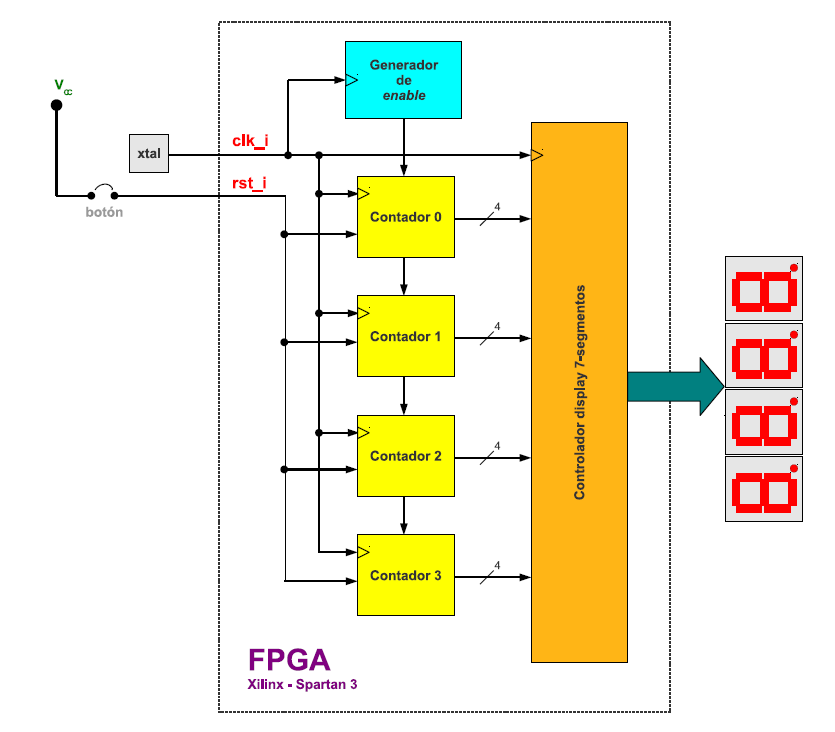
\includegraphics[scale=0.7]{arquitectura.png}\\[1cm] 
  \caption{Diagrama en bloques de la arquitectura propuesta.}
\end{figure}



\section{Contadores}

Los contadores de 2 y 4 bits se usan flip-flops D, ya que su diseño no era muy complejo. En cambio, para el contador de enable, por ejemplo, se uso un process.
Por su simpleza el contador de décadas se realizo usando un contador de 4 bits al que se le habilita el reset en el momento que este llega a 10.

\begin{figure}[h!]
  \centering
	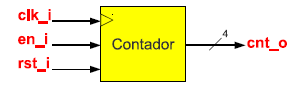
\includegraphics[scale=0.7]{contador.png}\\[1cm] 
  \caption{Contador BCD}
\end{figure}


\section{Controlador de display}

El controlador de display se implemento con una serie de ifs que habilitaban las salidas correspondientes según la entrada del contador. 

\begin{figure}[h!]
  \centering
	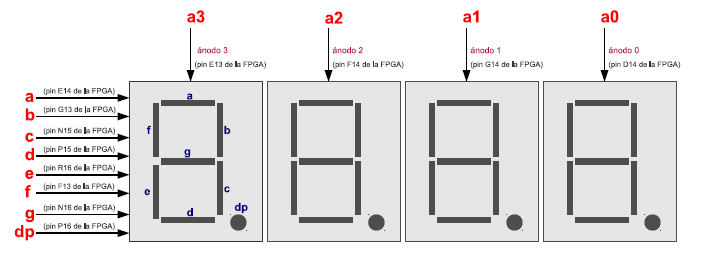
\includegraphics[scale=0.7]{display.png}\\[1cm] 
  \caption{Conexion entre las entradas y salidas de la FPGA y el display.}
\end{figure}

Este controlador se conecta al contador que se debe mostrar y estos van cambiando según el generador de enable, este generador cuenta hasta \( 50.000 \), es decir, tiene una frecuencia de \( 1 Khz \) si la frecuencia del micro es de \( 50 Mhz \).

\begin{figure}[h!]
  \centering
	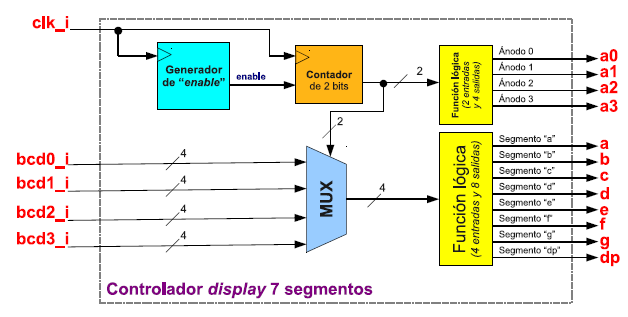
\includegraphics[scale=0.7]{controlador.png}\\[1cm] 
  \caption{Arquitectura para el controlador display 7 segmentos.}
\end{figure}


\section{Contador 9999}

Para juntar los 4 contadores y que cada uno vaya sumando correctamente se hizo que al llegar un dígito al valor 9 se le habilita el enable al siguiente numero, que este al comenzar en 0 pasa a 1 justo cuando el 9 paso al 0, esto se implemento para los 4 dígitos y se logro contar desde 0000 hasta 9999.


\section{Conclusion}

El presente trabajo sirvió para aprender tanto el lenguaje \( hdl \) como para sintetizar el código desarrollado en él en un kit FPGA.

\end{document}